\documentclass[a4paper, 12pt]{article}
\usepackage[a4paper,top=1.5cm, bottom=1.5cm, left=1cm, right=1cm]{geometry}
\usepackage[utf8]{inputenc}
\usepackage{mathtext}
\usepackage{amsmath}
\usepackage{amsfonts}
\usepackage[english, russian]{babel}
\usepackage{indentfirst}
\usepackage{longtable}
\usepackage{graphicx}
\graphicspath{{pictures/}}
\DeclareGraphicsExtensions{.pdf,.png,.jpg}
\usepackage{natbib}
\usepackage{hyperref}
\usepackage{subcaption}
\usepackage{emoji}
\babelfont{rm}{Droid Serif}
\babelfont{sf}{Droid Sans}
\renewcommand{\baselinestretch}{1.3}

\title{1.2.1.Определение скорости полета пули при помощи баллистического маятника}
\author{Платонов Егор. Б04-301}
\date{\today}

\begin{document}

\maketitle
\textbf{Цель работы:} определить скорость полета пули, применяя законы созранения и используя баллистические маятники.

\textbf{В работе используются:} духовое ружье на штативе, осветитель, оптическая система для измерения отклонений маятника, измерительная линейка, пули и весы для их взвенивания, а также баллистические маятники.

\section{Метод баллистического маятника, совершающего поступательное движение}

\begin{figure}[h]
    \centering
    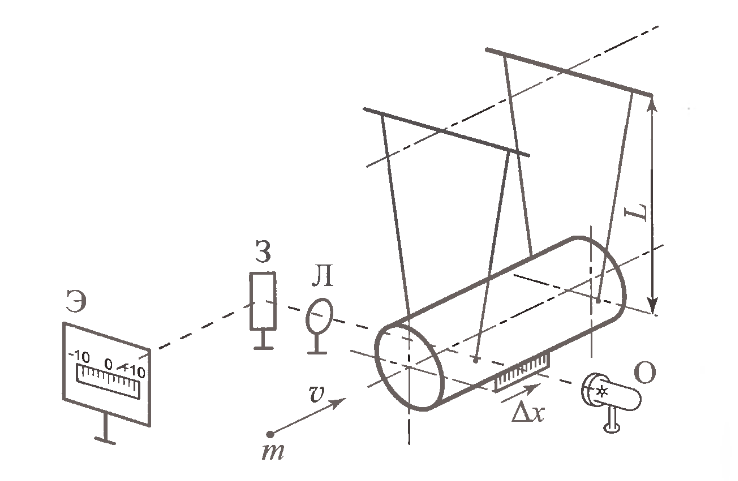
\includegraphics[scale=.5]{prop-1.png}
    \caption{Схема установки}
    \label{fig:enter-label}
\end{figure}

\begin{figure}[h]
    \centering
    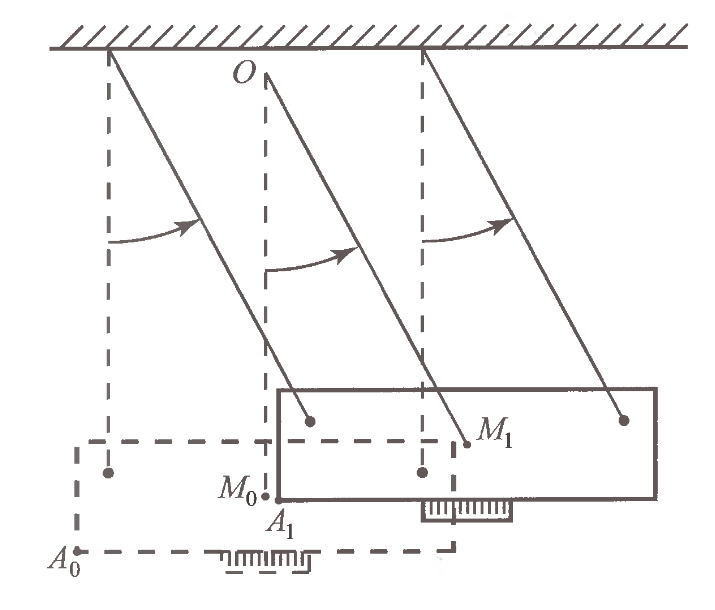
\includegraphics[scale=.5]{prop-2.png}
    \caption{Смещение баллистического маятника при попадании в него пули}
    \label{fig:enter-label}
\end{figure}

\begin{equation*}
    mv=(M+m)V
\end{equation*}
\begin{equation*}
    M >> m, v=\frac{M}{m}V
\end{equation*}
\begin{equation*}
    V^2=2gh=2gL(1-cos\phi)=4gLsin^2\frac{\phi}{2}=4gL\phi^2
\end{equation*}
\begin{equation*}
    \phi \approx \frac{\Delta x}{L}
\end{equation*}
\begin{equation*}
    v=\frac{M}{m}\sqrt{\frac{g}{L}}\Delta x
\end{equation*}



\end{document}
